\documentclass[pdftex,11pt,a4paper,titlepage]{report}
\usepackage[utf8]{inputenc}
\usepackage[english]{babel}
\usepackage[left=3cm,right=3cm,top=2cm,bottom=2cm]{geometry}
\usepackage[pdftex]{graphicx}
\usepackage{hyperref}
\usepackage{framed}

\newcommand{\HRule}{\rule{\linewidth}{0.5mm}}

\author{Tiago Lobato Gimenes}
\title{XCubeSat Controller}

\begin{document}

%------------------------------------------------------------%
%	Title Page
%------------------------------------------------------------%
\begin{titlepage}
\begin{center}

% Upper part of the page. The '~' is needed because \\
% only works if a paragraph has started.

\includegraphics[width=0.15\textwidth]{../images/CubeSat3.jpg}~\\[1cm]

\textsc{\LARGE X-CubeSat Controller}\\[1.5cm]

\textsc{\Large Version Pre-Beta}\\[0.5cm]

% Title
\HRule \\[0.4cm]
{ \huge \bfseries User Guide \\[0.4cm] }

\HRule \\[1.5cm]

% Author and supervisor
\begin{minipage}{0.4\textwidth}
\begin{flushleft} \large
\emph{Author:}\\
Tiago \textsc{L. Gimenes}
\end{flushleft}
\end{minipage}
\begin{minipage}{0.4\textwidth}
\begin{flushright} \large
\emph{Project Page:} \\
\url{https://github.com/tlgimenes/X-CubeSat}
\end{flushright}
\end{minipage}

\vfill

% Bottom of the page
{\large \today}

\end{center}
\end{titlepage}

%------------------------------------------------------------%
%	Table Of Contents
%------------------------------------------------------------%
\tableofcontents
\newpage

%------------------------------------------------------------%
%	Chapter - Requirements
%------------------------------------------------------------%
\chapter{Requirements}
\hspace{0.4cm} The current version of X-CubeSat Controller works only in POSIX compliant operating systems, like GNU/Linux, FreeBSD, etc, but future versions will work also in non POSIX compliant operating systems like Windows. You can find below the libraries and software needed to compile and run this version of XCubeSat Controller. The versions of the libraries and software below were tested, try other versions at your own risk.

\section{Basic Requirements}
\begin{itemize}
\item g++ version 4.7.2
\item GNU Make 3.81
\item Git version 1.7
\item GTK+3 
\item gtkmm version 3.0 or above
\item SQLite version 3.7.13
\item SQLite Wrapped version 1.3.1 \url{http://www.alhem.net/project/sqlite/}
\item Gpredict modified version that can be found in the following address \url{https://github.com/tlgimenes/gpredict} 
\end{itemize}

\section{Recommended Requirements}
\begin{itemize}
\item Hamlib version 1.2.15.3
\end{itemize}

\section{Warnings}
\begin{itemize}
\item It's absolutely necessary to use the modified version of Gpredict to realy be able to communicate with satellites, so do not download/install
the default version of Gpredict in distro repositories or from any official Gpredict site. 
\item For X-CubeSat Controller to work, the system needs to implement something called FIFO file. FIFO file is a type of file that allows the communication between Gpredict and X-CubeSat Controller, so if you are running a non POSIX compliant system, like Windows, it might not work or work as well as it does in a POSIX compliant system.
\end{itemize}

%------------------------------------------------------------%
%	Chapter - Install
%------------------------------------------------------------%
\chapter{Installation Instructions}
\hspace{0.4cm} The installation instructions will cover the compiling and installing phases. It will only shows how to install in the Debian GNU/Linux distribution but the same method should work in Ubuntu, Linux Mint and other Debian based distributions.

You can install this program in any directory that you want. For doing it 

\section{Installing dependencies}
\begin{itemize}
\item \textbf{Install g++}: Open a terminal and type:
\begin{framed}
\$ sudo apt-get install -y g++
\end{framed}
If you get no errors, you can go to the next item, otherwise google the problem.

\item \textbf{Install GNU Make}: In the same terminal type:
\begin{framed}
\$ sudo apt-get install -y make
\end{framed}
If you get no errors, you can go to the next item, otherwise google the problem.

\item \textbf{Install Git}: In the same terminal type:
\begin{framed}
\$ sudo apt-get install -y git
\end{framed}
If you get no errors, you can go to the next item, otherwise google the problem.

\item \textbf{Install gtkmm version 3.0}: In the same terminal type:
\begin{framed}
\$ sudo apt-get install -y libgtkmm-3.0-1 libgtkmm-3.0-dev libgtkmm-3.0-dbg
\end{framed}
If you get no errors, you can go to the next item, otherwise google the problem.

\item \textbf{Install SQLite version 3}: In the same terminal type:
\begin{framed}
\$ sudo apt-get install -y sqlite3
\end{framed}
If you get no errors, you can go to the next item, otherwise google the problem.

\item \textbf{Install SQLite Wrapped version 1.3.1}: Go the a directory that you want with the command \textbf{cd} and in the same terminal type:
\begin{framed}
\$ wget \url{http://www.alhem.net/project/sqlite/sqlitewrapped-1.3.1.tar.gz} \\
\$ tar -zxvf sqlitewrapped-1.3.1.tar.gz \\
\$ cd sqlitewrapped-1.3.1/ \\
\$ make \&\& make install
\end{framed}
If you get errors in this part, go to the url of the SQLite Wrapped project,\url{http://www.alhem.net/project/sqlite/download.html}, and follow their install instructions, sometimes the installation of this part is a little tricky. 

\item \textbf{Install Gpredict modified version}: Go the a directory that you want to install Gpredict with the command \textbf{cd} and in the same terminal type:
\begin{framed}
\$ sudo apt-get install libtool intltool \\
\$ git clone \url{https://github.com/tlgimenes/gpredict.git} \\
\$ cd gpredict \\
\$ sh autogen.sh \\
\$ ./configure \\
\$ make \&\& make install
\end{framed}
If you get errors in this part, go to the url of the Gpredict modified version project,\url{https://github.com/tlgimenes/gpredict}, and follow their install instructions, or read the \textbf{README} file provided with Gpredict, sometimes the installation of this part is a little tricky. 
\end{itemize}

\section{Compiling}
Usually if you got to this part, you should be ok to compile and install XCubeSat Controller. Open a terminal, go to the folder that you want to install XCubeSat Controller with the \textbf{cd} command and type:

\begin{framed}
\$ git clone \url{https://github.com/tlgimenes/X-CubeSat.git} \\
\$ cd X-CubeSat \\
\$ make \\
\$ cd dataBase \\
\$ sqlite3 XCubeSat\_Controller.db \\
.read tables.sql \\
.q
\end{framed}

Here you are ready to configure the XCubeSat\_ Controller \textbackslash o/.

%------------------------------------------------------------%
%	Chapter - Configure and Run
%------------------------------------------------------------%
\chapter{Configure and Run}
For X-CubeSat Controller to run, we need first to run Gpredict and if you want to use a rotator and/or a radio, you need to set Hamlib first.

In this session we are going first to configure a rotator, than a radio, than we are going to run Gpredict and finally we are going to run X-CubeSat Controller

First of all, we need to know the models of rotators that are supported and their ID. Open a terminal and type:
\begin{framed}
\$ rotctrl --list
\end{framed}

The output of this command is a list of rotator and models. Write down the value of the \textbf{Rig \#} column and type the following command.

\begin{framed}
\$ rotctrld -m "Model\_Value" -r "Serial\_Port" -t  "Port"
\end{framed}

Where 
\begin{itemize}
\item "Model\_Value" is the \textbf{Rig \#} value of the rotator that we found with the other command.
\item "Serial\_Port" is the name of the serial port connected to the rotator. Usually in Linux systems, the default port is located in /dev/ttyS0 or /dev/ttyUSB0 in the case of the use of USB to Serial adpters.
\item "Port" is the port that you want Hamlib to connect to. Pay attention in what port you put it to listen to, because Gpredict will ask the name of this port later. 
\end{itemize}

An example of this command for an Yaesu GS-232B connected in the serial port ttyS0 would be:
\begin{framed}
\$ rotctrld -m 603 -r /dev/ttyS0 -t 4533
\end{framed}

To configure a transceiver you basicaly need to do the same steps, so they won't be covered here. You can take a look in the Gpredict and Hamlib manuals for more configuration details.

Now that we have Hamlib running, it's time to set Gpredict. Open a new terminal and type:
\begin{framed}
\$ gpredict
\end{framed}
If the installation process worked well you are now runnig Gpredict. To configure the rotator and the transciever in Gpredict go to
\begin{framed}
edit $->$ preferences
\end{framed}

click in the \textbf{Interfaces} tab and add a new rotator and transciever with the port number that you passed in the "Port" parameter to Hamlib. 

To launch the tracking tool click in the down pointing arrow in the up right corner and select Antenna Control. It will open a new window with the satellites that you want to follow. 

Now, finaly we are going to launch XCubeSat Controller. To do so, open a new terminal and look for a folder called X-CubeSat with the "cd" and "ls" commands. Once you found the folder, enter in it and type:
\begin{framed}
\$ ./XCubeSat\_Controller
\end{framed}

Now you should be running the X-CubeSat Controller \textbackslash o/

%------------------------------------------------------------%
%	Chapter - Overview
%------------------------------------------------------------%
\chapter{Overview}
\hspace{0.4cm} The X-CubeSat Controller is a software for sending, receiving and stoking received data from the X-CubeSat and other satellites from a modem connected to a serial port to the computer. For each satellite we can program many scripts that are going to be put in a FIFO (first in first out) queue to be executed. The first script in the FIFO queue is executed when the satellite is above the horizon (calculated by Gpredict), than the script is reinserted in the last position of the FIFO queue and a new script is ready to be executed in the next pass of the satellite. 

The programming language is a simple, interpreted programming language that will allow to perform the act of sending, receiving and stoking data in the SQLite database. For more details about the programming language for this software, take a look in the others documents provided with this software. 

The X-CubeSat Controller is divided in many different frames that are going to be presented in the following chapters. Each frame has an specific function, from controlling the port that the modem will be connected to writing scripts and changing their priority. You can have a general view of the graphical interface in the figure \ref{GeneralView}.
\begin{figure}[h]
\centering
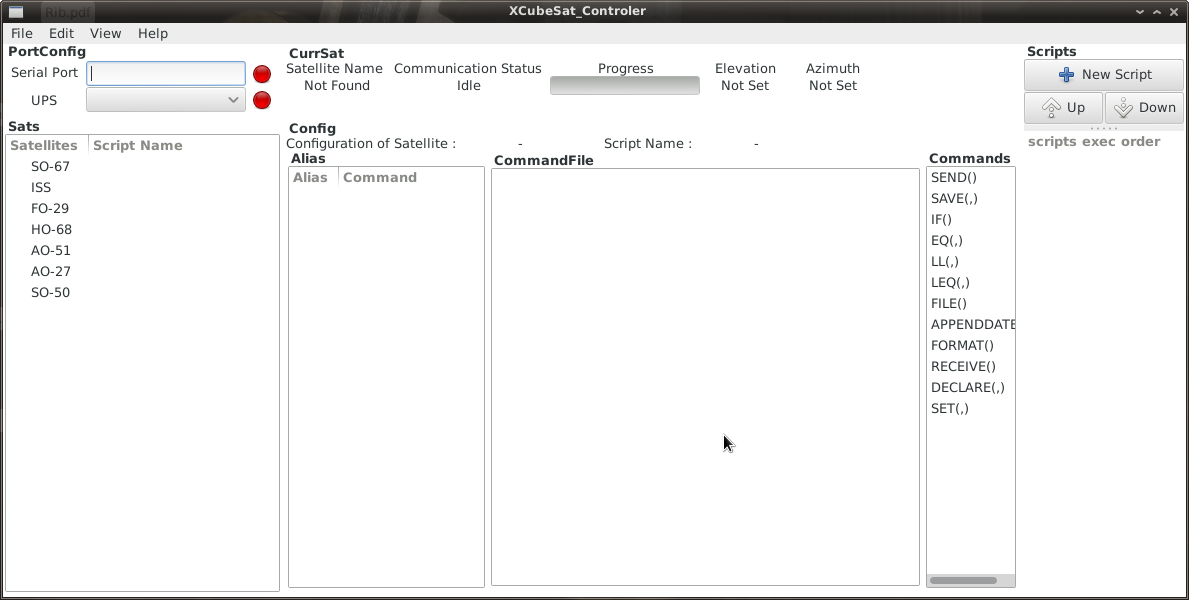
\includegraphics[scale=0.35]{../images/GeneralView.png}
\caption{General view of the graphical interface of X-CubeSat Controller}
\label{GeneralView}
\end{figure}

%------------------------------------------------------------%
%	Chapter - Port Config
%------------------------------------------------------------%
\chapter{Frame: Port Config}
\hspace{0.4cm} The port config frame can be seen in the figure \ref{PortConfigFrame}. This frame allows to change the serial port that the modem is connect to the computer and its speed.
\begin{figure}[h]
\centering
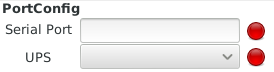
\includegraphics[scale=0.9]{../images/PortConfigFrame.png}
\caption{View of the PortConfig frame}
\label{PortConfigFrame}
\end{figure}

The red buttons that we can see in the figure above indicates the status of the port and its speed; green means that the serial port is connected and/or the speed for the port is supported and read means the opposite. You can see an example in the Figure \ref{PortConfigFrameGreen} that the serial port is connected and the speed is supported.

\begin{figure}[h]
\centering
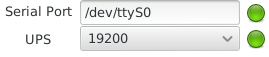
\includegraphics[scale=0.9]{../images/PortConfigFrameGreen.png}
\caption{View of the PortConfig frame green}
\label{PortConfigFrameGreen}
\end{figure}

In GNU/Linux systems the usual serial port is \textbf{/dev/ttyS0} for the motherboard ports and \textbf{/dev/ttyUSB0} for USB adapters. 

%------------------------------------------------------------%
%	Chapter - Sats
%------------------------------------------------------------%
\chapter{Frame: Sats}
\hspace{0.4cm} In the Sats frame you can find the satellites that are available in the current Gpredict configuration. If you add a new satellite in Gpredict, it wont be displayed until the next restart of this program.

In a tree path, we can see the scripts related to a satellite. You can rename them just by clicking over it and renaming it. Rename a script is essential for adding a new one, because a satellite cannot have two scripts with the same name. 

\textbf{Warning:} If the satellites shares a script with the same name with another satellite, there will be a race condition while saving the file and when re-opening then, one of them will be lost. 
\begin{figure}[h]
\centering
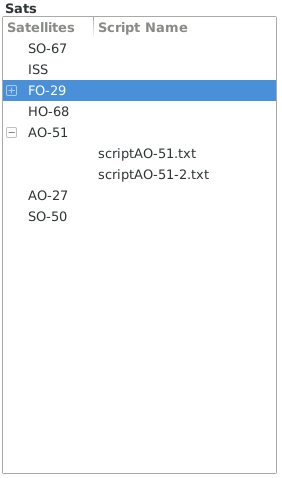
\includegraphics[scale=0.8]{../images/SatsFrame.png}
\caption{View of the Sats frame}
\label{SatsFrame}
\end{figure}

%------------------------------------------------------------%
%	Chapter - CurrSat
%------------------------------------------------------------%
\chapter{Frame: CurrSat}
\hspace{0.4cm} In the CurrSat frame you can find information concerning the next satellite that X-CubeSat Controller will run the scripts. 

The satellite name will appear as it is defined in Gpredict.

The fields elevation and azimuth shows the current elevation and azimuth of the satellite.

The field \textbf{Communication Status} can be \textbf{Idle} or \textbf{Communicating}, and it will change from \textbf{Idle} to \textbf{Communicating} when the script that is being executed asks for X-CubeSat Controller to send/receive data to/from the satellite.

The progress bar doesn't work yet in this version but it will show the progress while sending/receiving data to/from the satellite.
\begin{figure}[h]
\centering
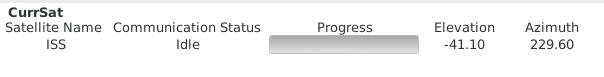
\includegraphics[scale=0.7]{../images/CurrSatFrame.png}
\caption{View of the CurrSats frame}
\end{figure}

%------------------------------------------------------------%
%	Chapter - Config
%------------------------------------------------------------%
\chapter{Frame: Config}

\hspace{0.4cm} In the config frame, you will be able to write and edit the script with the name in the field \textbf{Script Name} from the satellite with the name in the field \textbf{Configuration of Satellite}. In the figure \ref{ConfigFrame} you can see the complete frame.
\begin{figure}[h]
\centering
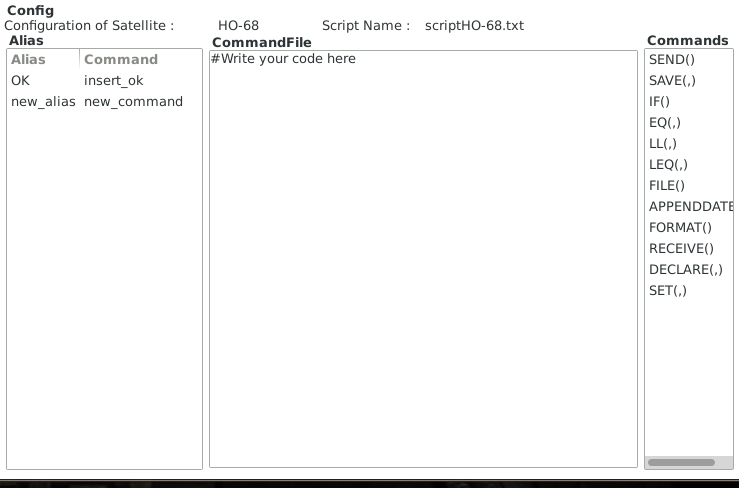
\includegraphics[scale=0.6]{../images/ConfigFrame.png}
\caption{View of the Config frame}
\label{ConfigFrame}
\end{figure}
%------------------------------------------------------------%
%	Section - Alias
%------------------------------------------------------------%
\section{Sub Frame: Alias}
\hspace{0.4cm} In the sub frame alias you can find the alias for the current script that is being edited. An alias allows the programmer to define "nicknames" for a standard command or to give names to constants.

An example of the use of an alias is to define the constant string that is going to be sent and than, instead of writing \textbf{SEND("12 32 42 25 d2 f4")} you can create an alias, and in the column \textbf{Alias} you can write \textbf{mode 1} with the corresponding column \textbf{Command} as \textbf{12 32 42 25 d2 f4} and than, write in the script \textbf{SEND("mode 1")}. It gives the code clearer and easier to understand. 

You can find a view of this frame in figure \ref{AliasSubFrame}.
\begin{figure}[h]
\centering
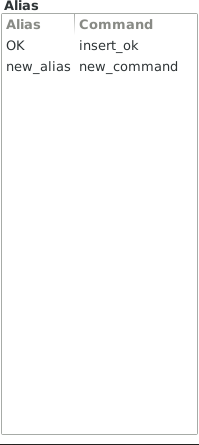
\includegraphics[scale=0.6]{../images/AliasSubFrame.png}
\caption{View of the Alias sub frame}
\label{AliasSubFrame}
\end{figure}

%------------------------------------------------------------%
%	Section - CommandFile
%------------------------------------------------------------%
\section{Sub Frame: CommandFile}
\hspace{0.4cm} The CommandFile frame is the text editor where you can write the script for the selected script for the selected satellite. 

You can find a view of this frame in figure \ref{CommandFileSubFrame}.

\begin{figure}[h]
\centering
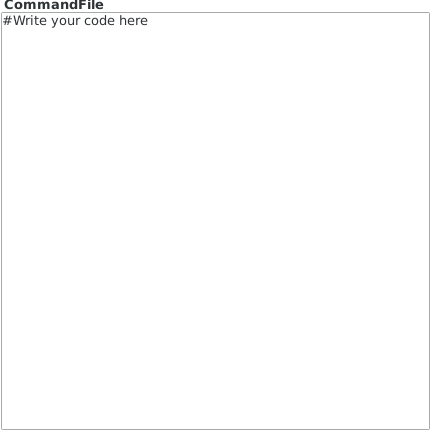
\includegraphics[scale=0.6]{../images/CommandFileSubFrame.png}
\caption{View of the CommandFile sub frame}
\label{CommandFileSubFrame}
\end{figure}
%------------------------------------------------------------%
%	Section - Commands
%------------------------------------------------------------%
\section{Sub Frame: Commands}
\hspace{0.4cm} In this frame you can find all the commands that can be written in the script. To add a certain command to the current script that is being edited, just double click in a row that the command will be added at the position of the cursor at the CommandFile frame. 

You can view this frame in figure \ref{CommandsSubFrame}

\begin{figure}[h]
\centering
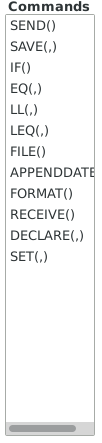
\includegraphics[scale=0.6]{../images/CommandsSubFrame.png}
\caption{View of the Commands sub frame}
\label{CommandsSubFrame}
\end{figure}
%------------------------------------------------------------%
%	Chapter - Scripts
%------------------------------------------------------------%
\chapter{Frame: Scripts}
\hspace{0.4cm} In the scripts frame you will be able to add a new script and to change their priority order in the FIFO queue. 

The button \textbf{New Script} adds a new script to the selected satellite. The new script created is named \textbf{new\_ script.txt} and it's highly recommended to rename the script for avoiding race conditions while saving the script, causing the lost of the script. 

The \textbf{UP} and \textbf{DOWN} buttons increase/decrease the priority of the selected script in the FIFO queue. 

You can view this frame in figure \ref{ScriptsFrame}.
\begin{figure}[h]
\centering
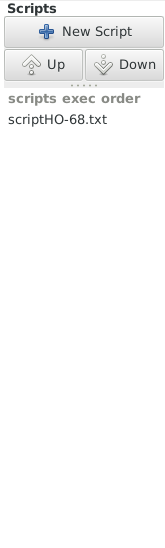
\includegraphics[scale=0.6]{../images/ScriptsFrame.png}
\caption{View of the Scripts sub frame}
\label{ScriptsFrame}
\end{figure}
%------------------------------------------------------------%
%	Section - Scripts Exec Order
%------------------------------------------------------------%
\section{Sub Frame: Scripts Exec Order}
The scripts exec order shows the execution order of the scripts. The higher is the script, closer it is of being executed.

%------------------------------------------------------------%
%	Chapter - Bug Issues
%------------------------------------------------------------%
\chapter{Bug Issue}
\begin{framed}
Oh NO ! X-CubeSat Controller just bugged !!!
\end{framed} 

If you just said the phrase above, don't worry ! X-CubeSat Controller is hosted by GitHub and it has an integrated Bug Issue Tracking system. If you have a new bug or issue and wants to tell it to the develpers go to the link: \url{https://github.com/tlgimenes/X-CubeSat/issues} and add a new issu, the XCubeSat Controller team will work as fast as possible to fix your issue, but for doing so, we need a good description of the bug and the executing conditions, so fill well the fields of the Bug Issue Tracker that we are going to do what we can to improve your experience with our software.

If you are an experienced C++ programmer, do not wait for us ! Make a pull request or fork the repository, it's free software ! Be Happy !

%------------------------------------------------------------%
\vspace{10cm}
\hspace{6cm}
\textbf{Enjoy your new XCubeSat Controller !}
\end{document}
